\documentclass[10pt]{article}
\usepackage[T1]{fontenc}
\usepackage{lmodern,amsmath,amssymb,booktabs,array,graphicx,tikz,pgfplots}
\usepackage[paperwidth=190mm,paperheight=224mm,margin=10mm]{geometry}
\usepackage[hidelinks]{hyperref}
\hypersetup{pdfauthor={},pdftitle={Monochrome mathematical illustrations: semiconductor-health identifiability}}
\usetikzlibrary{arrows.meta,positioning,calc,patterns}
\pgfplotsset{compat=1.18}
\newcommand{\trans}{^{\mathsf T}}\newcommand{\R}{\mathbb R}
\newcommand{\one}{\mathbf 1}\newcommand{\zero}{\mathbf 0}
\DeclareMathOperator{\rank}{rank}\DeclareMathOperator{\range}{range}
\DeclareMathOperator{\diag}{diag}\DeclareMathOperator{\Cov}{Cov}
\DeclareMathOperator{\Var}{Var}\DeclareMathOperator{\spanop}{span}
\newcommand{\FigureNote}{Visualization code prepared with assistance from OpenAI Codex.}
\pagestyle{empty}\setlength{\parindent}{0pt}
\tikzset{
 every picture/.style={font=\fontsize{9}{11}\selectfont,>=Latex},
 every node/.style={font=\fontsize{9}{11}\selectfont,inner sep=2pt},
 head/.style={font=\fontsize{9.5}{12}\selectfont\bfseries,anchor=west},
 tinytext/.style={font=\fontsize{8}{10}\selectfont},eq/.style={align=center},
 wire/.style={draw=black,line width=.5pt},arr/.style={->,black,line width=.65pt},
 device/.style={draw,fill=white,minimum width=1.1cm,minimum height=.38cm}}
\pgfplotsset{mathaxis/.style={axis lines=left,axis line style={black,line width=.5pt},
 tick style={black},tick label style={font=\fontsize{8}{10}\selectfont},
 label style={font=\fontsize{8.5}{10}\selectfont},grid=major,
 major grid style={black!15,line width=.2pt},
 legend style={font=\fontsize{8}{10}\selectfont,draw=none,fill=white},
 every axis plot/.append style={black}}}
\newcommand{\PlateTitle}[2]{\small\textbf{Mathematical plate #1}\hfill Monochrome TikZ / PGFPlots\par
 \vspace{1.5mm}{\large\bfseries #2}\par\vspace{2mm}}
\newcommand{\PlateCaption}[1]{\par\vspace{1mm}{\fontsize{8.5}{10.5}\selectfont #1\par
 \vspace{1mm}\FigureNote\par}}

\begin{document}
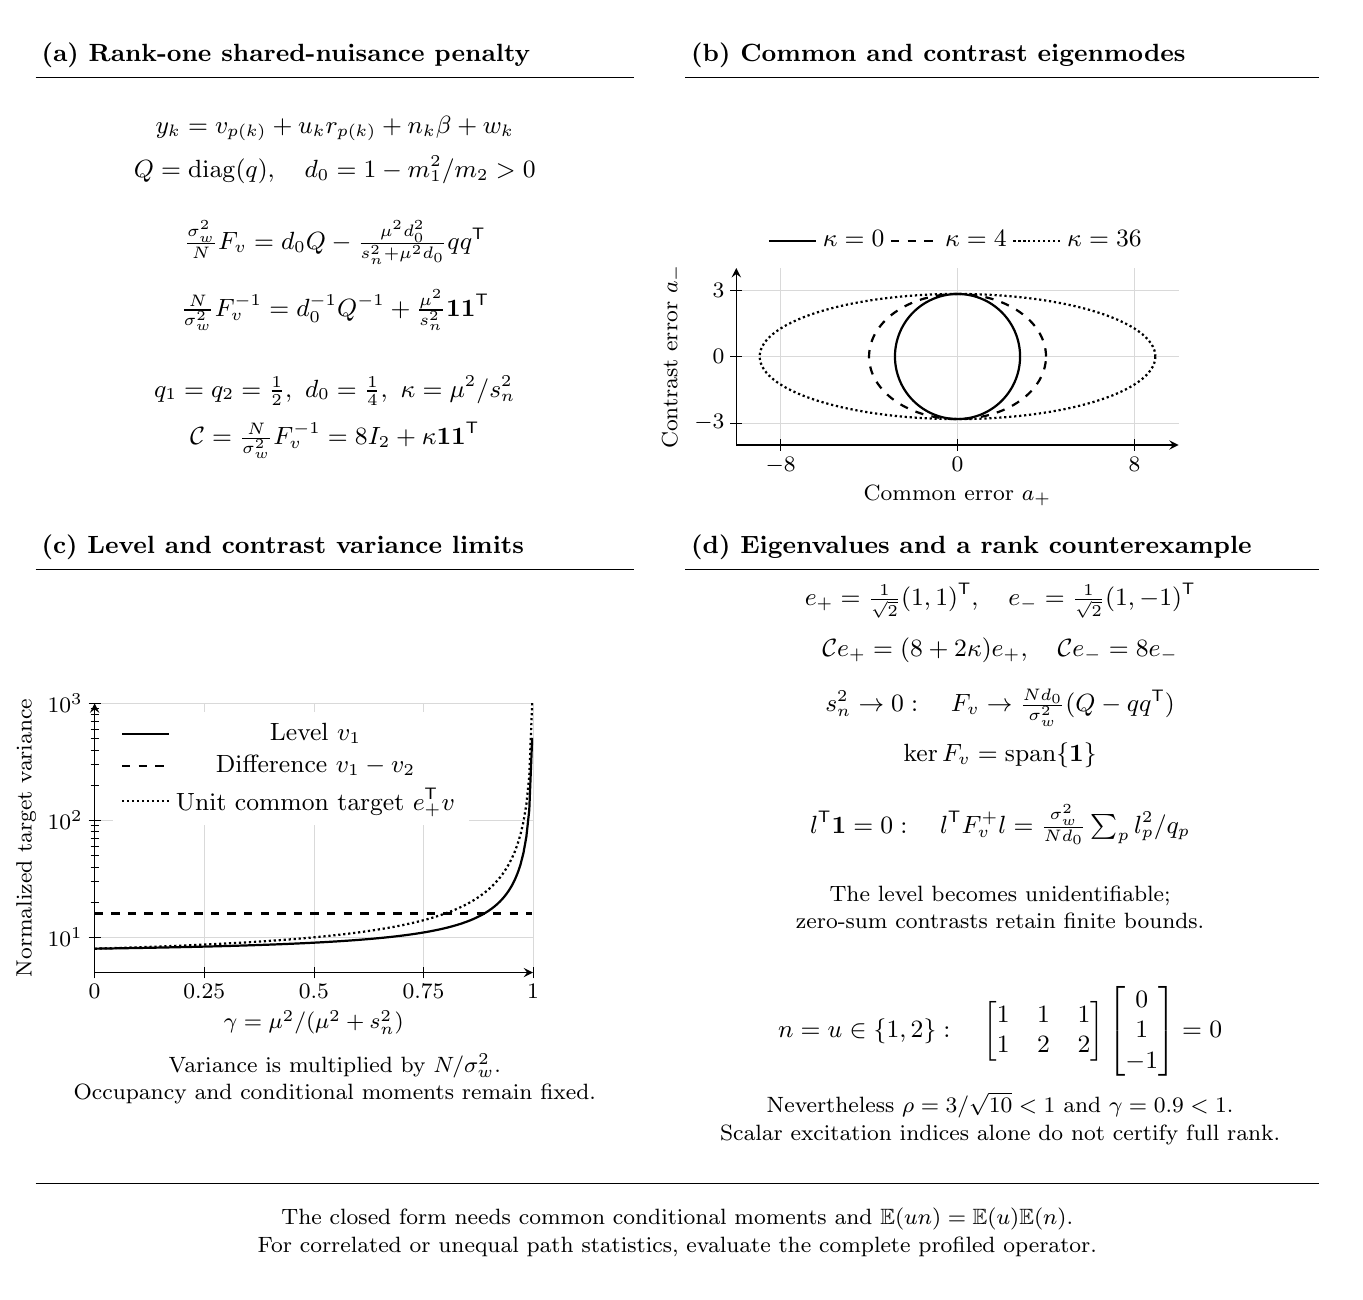
\begin{tikzpicture}[x=1cm,y=1cm]\path[use as bounding box] (0,0) rectangle (16.6,15.8);
\node[head] at (0.1,15.45){(a) Rank-one shared-nuisance penalty};\draw[wire] (0.1,15.17)--(7.699999999999999,15.17);
\node[head] at (8.35,15.45){(b) Common and contrast eigenmodes};\draw[wire] (8.35,15.17)--(16.4,15.17);
\node[eq] at (3.9,14.25){$y_k=v_{p(k)}+u_kr_{p(k)}+n_k\beta+w_k$\\[5pt]$Q=\diag(q),\quad d_0=1-m_1^2/m_2>0$};
\node[eq] at (3.9,12.65){$\frac{\sigma_w^2}{N}F_v=d_0Q-\frac{\mu^2d_0^2}{s_n^2+\mu^2d_0}qq\trans$\\[8pt]
$\frac{N}{\sigma_w^2}F_v^{-1}=d_0^{-1}Q^{-1}+\frac{\mu^2}{s_n^2}\one\one\trans$};
\node[eq] at (3.9,10.85){$q_1=q_2=\tfrac12,\ d_0=\tfrac14,\ \kappa=\mu^2/s_n^2$\\[5pt]
$\mathcal C=\frac{N}{\sigma_w^2}F_v^{-1}=8I_2+\kappa\one\one\trans$};
\begin{axis}[mathaxis,axis equal image,at={(9.0cm,10.5cm)},anchor=south west,width=7.2cm,height=4.2cm,
 xmin=-10,xmax=10,ymin=-4,ymax=4,xtick={-8,0,8},ytick={-3,0,3},
 xlabel={Common error $a_+$},ylabel={Contrast error $a_-$},legend style={at={(.5,1.03)},anchor=south,legend columns=3}]
\addplot[domain=0:360,samples=121,line width=.8pt] ({sqrt(8)*cos(x)},{sqrt(8)*sin(x)});\addlegendentry{$\kappa=0$}
\addplot[domain=0:360,samples=121,line width=.8pt,dashed] ({4*cos(x)},{sqrt(8)*sin(x)});\addlegendentry{$\kappa=4$}
\addplot[domain=0:360,samples=121,line width=.8pt,densely dotted] ({sqrt(80)*cos(x)},{sqrt(8)*sin(x)});\addlegendentry{$\kappa=36$}\end{axis}
\node[head] at (0.1,9.2){(c) Level and contrast variance limits};\draw[wire] (0.1,8.92)--(7.699999999999999,8.92);
\node[head] at (8.35,9.2){(d) Eigenvalues and a rank counterexample};\draw[wire] (8.35,8.92)--(16.4,8.92);
\begin{semilogyaxis}[mathaxis,at={(.85cm,3.8cm)},anchor=south west,width=7.15cm,height=5.0cm,
 xmin=0,xmax=1,ymin=5,ymax=1000,xtick={0,.25,.5,.75,1},ytick={10,100,1000},
 xlabel={$\gamma=\mu^2/(\mu^2+s_n^2)$},ylabel={Normalized target variance},legend style={at={(.04,.97)},anchor=north west}]
\addplot[domain=0:.998,samples=151,line width=.8pt]{8+x/(1-x)};\addlegendentry{Level $v_1$}
\addplot[domain=0:.998,samples=2,dashed,line width=.8pt]{16};\addlegendentry{Difference $v_1-v_2$}
\addplot[domain=0:.998,samples=151,densely dotted,line width=.8pt]{8+2*x/(1-x)};\addlegendentry{Unit common target $e_+\trans v$}\end{semilogyaxis}
\node[tinytext,align=center] at (3.9,2.45){Variance is multiplied by $N/\sigma_w^2$.\\Occupancy and conditional moments remain fixed.};
\node[eq] at (12.35,8.24){$e_+=\tfrac1{\sqrt2}(1,1)\trans,\quad e_-=\tfrac1{\sqrt2}(1,-1)\trans$\\[6pt]
$\mathcal C e_+=(8+2\kappa)e_+,\quad\mathcal C e_-=8e_-$};
\node[eq] at (12.35,6.9){$s_n^2\to0:\quad F_v\to\frac{Nd_0}{\sigma_w^2}(Q-qq\trans)$\\[5pt]$\ker F_v=\spanop\{\one\}$};
\node[eq] at (12.35,5.68){$l\trans\one=0:\quad l\trans F_v^+l=\frac{\sigma_w^2}{Nd_0}\sum_p l_p^2/q_p$};
\node[tinytext,align=center] at (12.35,4.63){The level becomes unidentifiable;\\zero-sum contrasts retain finite bounds.};
\node[eq] at (12.35,3.05){$n=u\in\{1,2\}:\quad\begin{bmatrix}1&1&1\\1&2&2\end{bmatrix}\begin{bmatrix}0\\1\\-1\end{bmatrix}=0$};
\node[tinytext,align=center] at (12.35,1.95){Nevertheless $\rho=3/\sqrt{10}<1$ and $\gamma=0.9<1$.\\Scalar excitation indices alone do not certify full rank.};
\draw[wire] (.1,1.12)--(16.4,1.12);
\node[tinytext,align=center] at (8.25,.5){The closed form needs common conditional moments and $\mathbb E(un)=\mathbb E(u)\mathbb E(n)$.\\For correlated or unequal path statistics, evaluate the complete profiled operator.};\end{tikzpicture}
\end{document}
